% FILLED (fill batch): process ④ Cooling — cyclotron / sympathetic scaling.
%   folds stdlib cyclotron_cool_bexponent / _bratio / _massspeedup (PR #1015)
%   + the Larmor P∝B² inversion + the giga-view mass speed-up + negative
%   controls, from companion/verify-ledger.json.
\section{Cooling --- Cyclotron and Sympathetic Cooling Scaling}
\label{app:cooling}

This appendix is the full data record for pipeline process
\textcircled{\scriptsize 4}. We derive the radiative (cyclotron) cooling time
constant $\tau_c\propto m^3/B^2$ from the Larmor radiated-power law
$P\propto B^2$, tabulate the field-ratio and the antiproton-vs-electron mass
speed-up, and pair each with its integer-exponent \tierBlue\ atom. Every
digit traces to PR~\#1015 (dimensional) / \#1094 (BLUE-MAX) and the atoms in
\texttt{companion/verify-ledger.json}.

% -------------------------------------------------------------------------
\subsection{The cooling-time scaling from Larmor radiation}
\label{app:cool-deriv}

A charged particle of mass $m$ and charge $q$ gyrating in field $B$ has
cyclotron frequency $\omega_c=qB/m$ and, at transverse speed $v_\perp$,
centripetal acceleration $a=\omega_c v_\perp$. By the Larmor formula it
radiates power
\begin{equation}
P \;=\; \frac{q^2 a^2}{6\pi\varepsilon_0 c^3}
   \;=\; \frac{q^2}{6\pi\varepsilon_0 c^3}\,\omega_c^2\,v_\perp^2
   \;=\; \frac{q^4 B^2}{6\pi\varepsilon_0 c^3\, m^2}\,v_\perp^2 .
\label{eq:cool-larmor}
\end{equation}
The transverse kinetic energy is $E_\perp=\tfrac12 m v_\perp^2$, so it decays
as $\dot E_\perp = -P \propto -(B^2/m^2)\,E_\perp/m = -(B^2/m^3)E_\perp$,
i.e.\ exponentially with time constant
\begin{equation}
\boxed{\;\tau_c \;\propto\; \frac{m^3}{B^{2}}\;}.
\label{eq:cool-tau}
\end{equation}
The two integer exponents are the load-bearing claim: the cooling time falls
as the \emph{square} of the field and rises as the \emph{cube} of the mass.
These are exact BLUE-MAX integer atoms
(\verb|cyclotron_cool_bexponent|$=-2$, \verb|cyclotron_cool_massexponent|$=3$;
Appendix~\ref{app:bluemax}). The normalized field scaling
$\tau_c(B)/\tau_c(1\,\mathrm{T})=B^{-2}$, its registered anchor, and the
discriminating wrong-slope control are plotted in Fig.~\ref{fig:cool-b2}.

\begin{figure}[h]
\centering
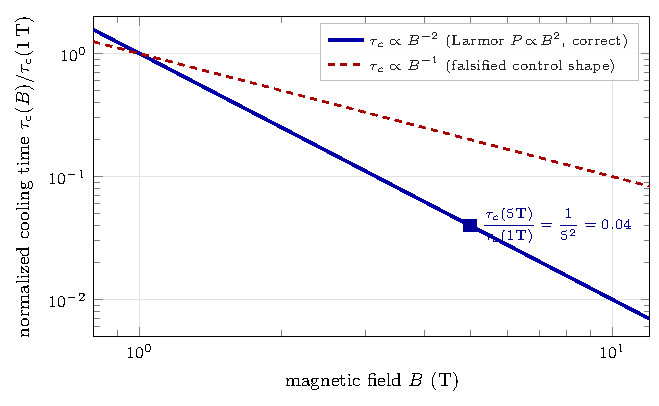
\includegraphics[width=0.82\linewidth]{figures/fig07_cooling_b2.pdf}
\caption{Cyclotron cooling time versus field, normalized to $1$\,T (log--log).
The correct $\tau_c\propto B^{-2}$ scaling (blue) passes exactly through the
registered anchor $\tau_c(5\,\mathrm{T})/\tau_c(1\,\mathrm{T})=1/5^2=0.04$
(\texttt{cyclotron\_cool\_bratio}, PR~\#1015). The dashed red line is the
implied shape of the falsified $B^{-1}$ control, plotted so the $-2$-vs-$-1$
discrimination is visible. Only the single registered ratio anchor is a
verify atom; the curves are the exact scaling laws, not fitted to data
(commons @D~g3).}
\label{fig:cool-b2}
\end{figure}

% -------------------------------------------------------------------------
\subsection{The antiproton-vs-electron mass penalty}
\label{app:cool-mass}

The $m^3$ dependence is why \emph{direct} cyclotron cooling of an antiproton
is impractical: with $m_{\bar p}/m_e\approx1836$, the bare antiproton cooling
time is $\approx1836^3\approx6.19\times10^9$ times longer than an electron's
at the same field. Because $6.19\times10^9$ overflows the discriminating
$\varepsilon=10^{-9}$ gate at unit scale, the kernel registers the giga-view
\verb|cyclotron_cool_massspeedup| which returns the mass ratio cubed in a
$10^{-9}$-scaled view ($\approx6.19051$). This $\sim$6-billion-fold penalty
is exactly why real experiments cool $\bar p$ \emph{sympathetically} ---
co-trapping a cloud of electrons (which cool fast by Eq.~\eqref{eq:cool-tau})
and letting Coulomb collisions thermalize the antiprotons to the electron
temperature. The funnel closes the \emph{scaling} that motivates this choice,
not the sympathetic-cooling rate itself.

\begin{table}[h]
\centering
\small
\setlength{\tabcolsep}{5pt}
\begin{tabular}{@{}l l r r r l@{}}
\toprule
\textbf{atom} & \textbf{args} & \textbf{expected} & \textbf{observed} & $|\Delta|$ & \textbf{tier} \\
\midrule
\verb|cyclotron_cool_bexponent|    & (0)               & $-2$    & $-2$    & $0$                 & \tierBlue \\
\verb|cyclotron_cool_massexponent| & ()                & $3$     & $3$     & $0$                 & \tierBlue \\
\verb|cyclotron_cool_bratio_exponent| & ()             & $2$     & $2$     & $0$                 & \tierBlue \\
\verb|cyclotron_cool_bratio|       & (5.0,1.0)         & $0.04$  & $0.04$  & $6.9\times10^{-18}$ & \tierGreen \\
\verb|cyclotron_cool_massspeedup|  & ($m_{\bar p},m_e$) & $6.19051$ & $6.19051$ & $1.4\times10^{-14}$ & \tierGreen \\
\bottomrule
\end{tabular}
\caption{Process \textcircled{\scriptsize 4} cooling atoms
(\texttt{companion/verify-ledger.json}, PR~\#1015 / \#1094). The three
\tierBlue\ integer atoms attest the exponents of Eq.~\eqref{eq:cool-tau}; the
two \tierGreen\ atoms attest the dimensional field ratio
($1/5^2=0.04$) and the $10^{-9}$-scaled mass speed-up
(raw $\approx6.19\times10^9$).}
\label{tab:cool-verify}
\end{table}

\begin{lstlisting}
verify --expr cyclotron_cool_bratio(5.0,1.0)=0.04
  calc   = 0.0400000 ~ expected 0.04 (|Delta|=6.94e-18 <= eps=1e-9)
  tier   = SUPPORTED-NUMERICAL (hexa-native libm-class recompute)
verify --expr cyclotron_cool_bexponent(0)=-2
  calc   = -2 == expected -2 (|Delta|=0)
  tier   = SUPPORTED-FORMAL (integer algebraic-root identity)
verify --expr cyclotron_cool_bexponent(0)=-3   # negative control
  calc   = -2 != expected -3 (|Delta|=1 > eps=1e-9)
  tier   = FALSIFIED (controlled negative)
\end{lstlisting}

% -------------------------------------------------------------------------
\subsection{Negative controls}
\label{app:cool-controls}

Two deterministic controls return \textsc{Falsified}: a wrong field-exponent
($-3$ instead of $-2$) and a wrong field ratio ($0.1$ instead of $0.04$, i.e.\
the $B^{-1}$ shape of Fig.~\ref{fig:cool-b2}). They confirm the verifier
distinguishes the correct $B^{-2}$ law from nearby wrong powers.

% -------------------------------------------------------------------------
\subsection{Honest scope}
\label{app:cool-scope}

This appendix closes the cooling-time \emph{scaling} ($\tau_c\propto B^{-2}$,
$m^3$), not an absolute cooling time in seconds nor an equilibrium
temperature. The absolute $\tau_c$ carries a prefactor
($6\pi\varepsilon_0 m^3 c^3/q^4$) and depends on geometry; the equilibrium
$T$ is set by the balance of cooling against heating mechanisms (RF noise,
collisions, expansion) that are apparatus-specific and out of scope. The
$\bar p$-vs-$e^-$ speed-up uses the CODATA-2018 masses
\citep{mohr2018codata}; CPT supplies $m_{\bar p}=m_p$.
